\documentclass[journal,10pt,twocolumn]{IEEEtran}
\usepackage[utf8]{inputenc}
\usepackage{amsmath,amssymb,amsfonts}
\usepackage{graphicx}
\usepackage{booktabs}
\usepackage{url}
\usepackage{tikz}
\usetikzlibrary{shapes,arrows,positioning}
\usepackage{subcaption}
\usepackage{algorithm}
\usepackage{algorithmic}

\begin{document}

\title{Introduction to Robotics - Final Project}
\author{Mauro Antonio de Palma - 256175}

\maketitle

\section{Introduction}

\subsection{Problem Statement}
The challenge for this project lies in designing a control system that can:
\begin{itemize}
	\item Track complex spatial trajectories with high accuracy
	\item Maintain tool orientation constraints (perpendicular to surface)
	\item Optimize robot configuration for enhanced dexterity
	\item Handle kinematic redundancy effectively.
\end{itemize}

\subsection{System Overview}
This solution employs an 8-DoF redundant manipulator combining: (i) 2-DoF Pan-Tilt Platform for additional workspace and mobility, (ii) 6-DoF Unitree Z1 Arm for precise manipulation capabilities, (iii) Task-Space Controller for accurate pose tracking, and (iv) Null-Space Optimization for manipulability maximization using redundancy.

The robot executes a horizontal circular trajectory (radius 0.20 m) at constant height above the table, with the tool z-axis maintained perpendicular to the surface for effective cleaning.

\section{Robot Kinematics and Dynamics}

\subsection{Kinematic Structure}
The robot consists of 8 revolute joints arranged in the following kinematic chain:

\begin{equation}
	\begin{aligned}
		\text{World} &\rightarrow \text{Platform}_{\text{roll}} \rightarrow \text{Platform}_{\text{pitch}} \\
		&\rightarrow \text{Z1}_{\text{joint1}} \rightarrow \cdots \rightarrow \text{Z1}_{\text{joint6}} \rightarrow \text{Tool Tip}
	\end{aligned}
\end{equation}

The joint vector $\mathbf{q} \in \mathbb{R}^8$ is defined as:
\begin{equation}
\mathbf{q} = [q_0, q_1, q_2, q_3, q_4, q_5, q_6, q_7]^T
\end{equation}
where $q_0, q_1$ are platform joints and $q_2$ through $q_7$ are Z1 arm joints.

\textbf{Implementation Link:} This structure is defined in URDF file \texttt{assembly.urdf} and loaded using \texttt{pinocchio.buildModelFromUrdf()} in \texttt{robot\_model.py}.

\subsection{Forward Kinematics}
The forward kinematics function maps joint positions to end-effector pose:
\begin{equation}
\mathbf{x} = f(\mathbf{q}) = \begin{bmatrix} \mathbf{p}(\mathbf{q}) \\ \mathbf{R}(\mathbf{q}) \end{bmatrix}
\end{equation}
where $\mathbf{p} \in \mathbb{R}^3$ is the position and $\mathbf{R} \in SO(3)$ is the rotation matrix.

\textbf{Implementation Link:} In the project I used the features provided by Pinocchio's APIs. It can read the model and perform forward kinematics calculations in an very optimized way also thanks to the parameters reduction given by the Denavit-Hartenberg convention.

\subsection{Jacobian Analysis}
The geometric Jacobian relates joint velocities to end-effector twist:
\begin{equation}
\dot{\mathbf{x}} = \mathbf{J}(\mathbf{q})\dot{\mathbf{q}} = \begin{bmatrix} \mathbf{J}_p(\mathbf{q}) \\ \mathbf{J}_o(\mathbf{q}) \end{bmatrix}\dot{\mathbf{q}}
\end{equation}
where $\mathbf{J}_p \in \mathbb{R}^{3 \times 8}$ is the position Jacobian and $\mathbf{J}_o \in \mathbb{R}^{3 \times 8}$ is the orientation Jacobian.

The Jacobian time derivative $\dot{\mathbf{J}}$ is computed as:
\begin{equation}
\dot{\mathbf{J}}(\mathbf{q}, \dot{\mathbf{q}}) = \frac{\partial \mathbf{J}}{\partial \mathbf{q}}\dot{\mathbf{q}}
\end{equation}

\textbf{Implementation Link:} I compute the Jacobian using \texttt{pinocchio.computeJointJacobians} and extract the frame Jacobian with \texttt{pinocchio.getFrameJacobian}. The term $\dot{\mathbf{J}}\dot{\mathbf{q}}$ is computed analytically using \texttt{pinocchio.getFrameClassicalAcceleration} in the \texttt{get\_jacobian\_derivative} method, which is more efficient than numerical finite differences.

\subsection{Robot Dynamics}
The dynamic model follows the Euler-Lagrange formulation:
\begin{equation}
\mathbf{M}(\mathbf{q})\ddot{\mathbf{q}} + \mathbf{C}(\mathbf{q}, \dot{\mathbf{q}})\dot{\mathbf{q}} + \mathbf{g}(\mathbf{q}) = \boldsymbol{\tau}
\end{equation}
where $\mathbf{M}(\mathbf{q}) \in \mathbb{R}^{8 \times 8}$ is the mass/inertia matrix, $\mathbf{C}(\mathbf{q}, \dot{\mathbf{q}})\dot{\mathbf{q}} \in \mathbb{R}^8$ represents Coriolis and centrifugal forces, $\mathbf{g}(\mathbf{q}) \in \mathbb{R}^8$ is the gravity vector, and $\boldsymbol{\tau} \in \mathbb{R}^8$ are joint torques.

The bias forces combine Coriolis and gravity terms:
\begin{equation}
\mathbf{h}(\mathbf{q}, \dot{\mathbf{q}}) = \mathbf{C}(\mathbf{q}, \dot{\mathbf{q}})\dot{\mathbf{q}} + \mathbf{g}(\mathbf{q})
\end{equation}

\textbf{Implementation Link:} I compute all dynamic quantities using Pinocchio: \texttt{pinocchio.crba} for the mass matrix, \texttt{pinocchio.nonLinearEffects} for bias forces, and \texttt{pinocchio.computeAllTerms} for efficient batch computation in \texttt{RobotModel} class.

\section{Manipulability Analysis}

\subsection{Manipulability Measure}
For redundant manipulators, manipulability quantifies the dexterity and conditioning of the robot configuration. Following Yoshikawa's definition \cite{yoshikawa1985}:
\begin{equation}
w(\mathbf{q}) = \sqrt{\det(\mathbf{J}_p\mathbf{J}_p^T)}
\end{equation}

This measure indicates how much room for movement the robot has to perform its tasks. Higher manipulability indicates: 
\begin{itemize}
	\item Better ability to move in all directions
	\item Improved force transmission capabilities
	\item Enhanced robustness to singularities
\end{itemize}

\textbf{Implementation Link:} I implement this in the \texttt{compute\_yoshikawa\_manipulability} method adding an additional small damping factor to maintain numerical stability

\subsection{Manipulability Gradient}
To optimize manipulability, the controller computes its gradient with respect to joint positions:
\begin{equation}
\nabla w(\mathbf{q}) = \frac{\partial w}{\partial \mathbf{q}} \in \mathbb{R}^8
\end{equation}

Using finite differences for numerical computation:
\begin{equation}
\frac{\partial w}{\partial q_i} \approx \frac{w(\mathbf{q} + \epsilon) - w(\mathbf{q})}{\epsilon}
\end{equation}
where $\epsilon$ is a small perturbation on \textit{i}-th joint that impacts the whole robot system.

\textbf{Implementation Link:} I implement this gradient computation in \texttt{compute\_manipulability\_gradient()} method using a perturbation value of $\epsilon = 1e-4$

\section{Task-Space Control Design}

\subsection{Control Objective}
The primary control objective is to track a time-varying reference trajectory $\mathbf{x}_d(t)$ while maintaining tool orientation constraints. The tracking error is defined as:
\begin{equation}
\mathbf{e}(t) = \mathbf{x}_d(t) - \mathbf{x}(t)
\end{equation}

For pose control, we separate position and orientation errors:
\begin{equation}
\mathbf{e} = \begin{bmatrix} \mathbf{e}_p \\ \mathbf{e}_o \end{bmatrix} = \begin{bmatrix} \mathbf{p}_d - \mathbf{p} \\ \log(\mathbf{R}_d\mathbf{R}^T) \end{bmatrix}
\end{equation}
where $\log(\cdot)$ denotes the SO(3) logarithm map for orientation error.

\textbf{Implementation Link:} I compute position error as \texttt{pose\_desired.translation - pose\_current.translation} and orientation error using \texttt{pinocchio.log3(R\_desired @ R\_current.T)} where the rotation error matrix is computed before applying the SO(3) logarithm map.

\subsection{Inverse Dynamics Control}
The task-space inverse dynamics controller computes the required joint accelerations:
\begin{equation}
\ddot{\mathbf{q}} = \mathbf{J}^\#(\mathbf{q})\left[\ddot{\mathbf{x}}_d + \mathbf{K}_d\dot{e} + \mathbf{K}_p\mathbf{e} - \dot{\mathbf{J}}\dot{\mathbf{q}}\right]
\end{equation}

where $\mathbf{J}^\#$ is the damped pseudoinverse:
\begin{equation}
\mathbf{J}^\# = \mathbf{J}^T(\mathbf{J}\mathbf{J}^T + \lambda^2\mathbf{I})^{-1}
\end{equation}

The control gains $\mathbf{K}_p, \mathbf{K}_d \in \mathbb{R}^{6 \times 6}$ are diagonal matrices providing PD control in task space.

\textbf{Implementation Link:} I implement this in \texttt{calculate\_primary\_task} method invoked by the control loop. $\mathbf{J}^\#$ is calculated by \texttt{damped\_pseudo\_inverse} method with adaptive damping $\lambda$ based on the current manipulability condition (higher factor for lower manipulabilities).

\subsection{Null-Space Optimization}
For redundant robots ($n > m$, where $n=8$ DOFs and $m=6$ task dimensions), we exploit the null space to achieve secondary objectives without affecting the primary task.

The null-space projector is:
\begin{equation}
\mathbf{N} = \mathbf{I} - \mathbf{J}^\#\mathbf{J}
\end{equation}

The total joint acceleration combines primary and secondary tasks:
\begin{equation}
\ddot{\mathbf{q}} = \ddot{\mathbf{q}}_{\text{task}} + \ddot{\mathbf{q}}_{\text{null}}
\end{equation}

For manipulability maximization:
\begin{equation}
\ddot{\mathbf{q}}_{\text{null}} = k_{\text{null}}\mathbf{N}\nabla w(\mathbf{q})
\end{equation}

\textbf{Implementation Link:} I implement null-space optimization in controller with gain $k_{\text{null}} = 2.0$ and dynamic adjustment based on tracking performance. The null-space projector is computed using \texttt{numpy.eye(8) - J\_pinv @ J}.

\subsection{Complete Control Law}
The final control torque is computed using inverse dynamics:
\begin{equation}
\boldsymbol{\tau} = \mathbf{M}(\mathbf{q})\ddot{\mathbf{q}} + \mathbf{h}(\mathbf{q}, \dot{\mathbf{q}})
\end{equation}

\textbf{Implementation Link:} I compute the final torque in \texttt{compute\_control} method using \texttt{self.robot.mass\_matrix(q) @ ddq + self.robot.bias\_forces(q, dq)} and apply torque limits for safety.

\section{Trajectory Generation}

\subsection{Circular Trajectory}
The task requires tracking a horizontal circle with constant height. The trajectory parameters are:

\begin{itemize}
	\item Center: $\mathbf{p}_c = [0.35, 0.0, 0.05]$ m
	\item Radius: $r = 0.20$ m
	\item Angular velocity: $\omega = 1$ rad/s
	\item Height above table: $z = 0.05$ m
\end{itemize}

The position reference is:
\begin{equation}
\mathbf{p}_d(t) = \mathbf{p}_c + \begin{bmatrix} r\cos(\omega t) \\ r\sin(\omega t) \\ 0 \end{bmatrix}
\end{equation}

The orientation reference maintains the tool perpendicular to the table. To keep the Z-axis pointing downwards it rotates the end-effector on the X-axis by 180° ($\pi$ rad)
\begin{equation}
\mathbf{R}_d = \begin{bmatrix} 1 & 0 & 0 \\ 0 & cos(\pi) & -sin(\pi) \\ 0 & sin(\pi) & cos(\pi) \end{bmatrix}
\end{equation}

The velocity and acceleration profiles are obtained analytically from the position first and second order derivatives:

Velocity:
\begin{equation}
	\dot{\mathbf{p}}_d(t) = \begin{bmatrix} -r\omega\sin(\omega t) \\ r\omega\cos(\omega t) \\ 0 \end{bmatrix}
\end{equation}

Acceleration:
\begin{equation}
	\ddot{\mathbf{p}}_d(t) = \begin{bmatrix} -r\omega^2\cos(\omega t) \\ -r\omega^2\sin(\omega t) \\ 0 \end{bmatrix}
\end{equation}

\textbf{Implementation Link:} I implement these concepts in \texttt{CircularTrajectory} class with methods \texttt{get\_pose()}, \texttt{get\_twist()}, and \texttt{get\_acceleration()} that return the complete reference trajectory at any time $t$.

\subsection{Approach Phase}
To smoothly transition from the initial configuration to the circular trajectory, I use a quintic polynomial trajectory:
\begin{equation}
s(t) = 10t^3 - 15t^4 + 6t^5
\end{equation}
where $s(t) \in [0,1]$ is the interpolation parameter with zero velocity and acceleration at boundaries.

The interpolated pose during approach is:
\begin{equation}
\mathbf{x}_d(t) = \mathbf{x}_{\text{start}} + s(t) (\mathbf{x}_{\text{circle}} - \mathbf{x}_{\text{start}})
\end{equation}

The rotation interpolation is performed using the \textbf{SLERP} (Spherical Linear Interpolation) to ensure smooth orientation transitions with constant angular velocity along the shortest path on the unit sphere.

While trapezoidal velocity profiles are commonly used for their simplicity, the quintic polynomial trajectory is preferred because it eliminates \textit{jerk} (discontinuities in acceleration) at the start and end points. The trapezoidal profile creates abrupt acceleration changes at velocity transitions, whereas the quintic polynomial ensures continuous acceleration with zero jerk at boundaries, resulting in smoother robot motion and reduced mechanical stress.

\textbf{Implementation Link:} I implement this in \texttt{PointToPointTrajectory} class using quintic polynomial coefficients and blend it with the circular trajectory in \texttt{CleaningTrajectory} class, which manages the complete approach + cleaning motion sequence.

\section{Implementation and Results}

\subsection{System Architecture}
The implementation uses Python 3.8 with the Pinocchio robotics library for kinematic and dynamic computations, running on Ubuntu 20.04 in a VirtualBox VM for compatibility. The modular architecture consists of:

\begin{itemize}
	\item \texttt{robot\_model.py}: URDF loading, forward/inverse kinematics, dynamics
	\item \texttt{controller.py}: Task-space controller with null-space optimization
	\item \texttt{trajectory.py}: Reference trajectory generation
	\item \texttt{run\_sim.py}: Main simulation loop and data logging
\end{itemize}

\begin{table}[H]
\centering
\caption{Controller Parameters}
\begin{tabular}{lc}
\toprule
Parameter & Value \\
\midrule
Approach gain $K_{p,pos}$ & 800.0 \\
Approach derivative gain $K_{d,pos}$ & 56.57 \\
Orientation gain $K_{p,rot}$ & 600.0 \\
Derivative gain $K_{d,rot}$ & 48.99 \\
Null-space gain $k_{null}$ & 5.0 \\
Damping factor $\lambda$ & 0.1 \\
Simulation time step & 1 ms \\
\bottomrule
\end{tabular}
\end{table}

\subsection{Results and Visualization}

\subsubsection{Trajectory Tracking Performance}
The trajectory tracking performance is evaluated through quantitative metrics and visual analysis. Fig.~\ref{fig:robot_main} shows the 3D trajectory comparison between reference and actual end-effector paths, demonstrating a good tracking with the null-space optimization enabled and the orientation requirement for the end-effector.

The top-view trajectory in Fig.~\ref{fig:trajectory_xy} reveals circular tracking with some deviation from the desired 20 cm radius path. The blue trajectory (actual robot motion) closely follows the green reference trajectory, increasing the error close to singularity zone.

\begin{figure}[h]
	\centering
	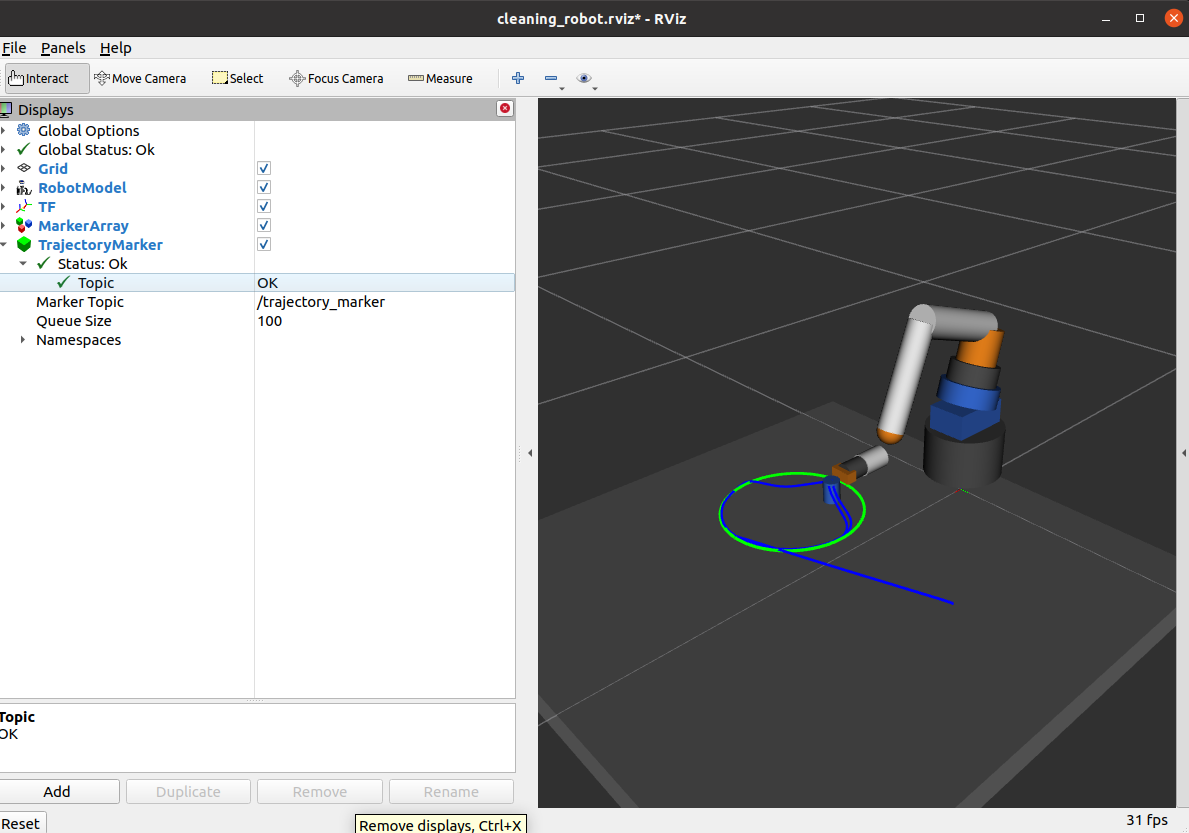
\includegraphics[width=0.7\columnwidth]{images/manipulability.png}
	\caption{Final robot trajectory with manipulability optimization}
	\label{fig:robot_main}
\end{figure}

\begin{figure}[h]
	\centering
	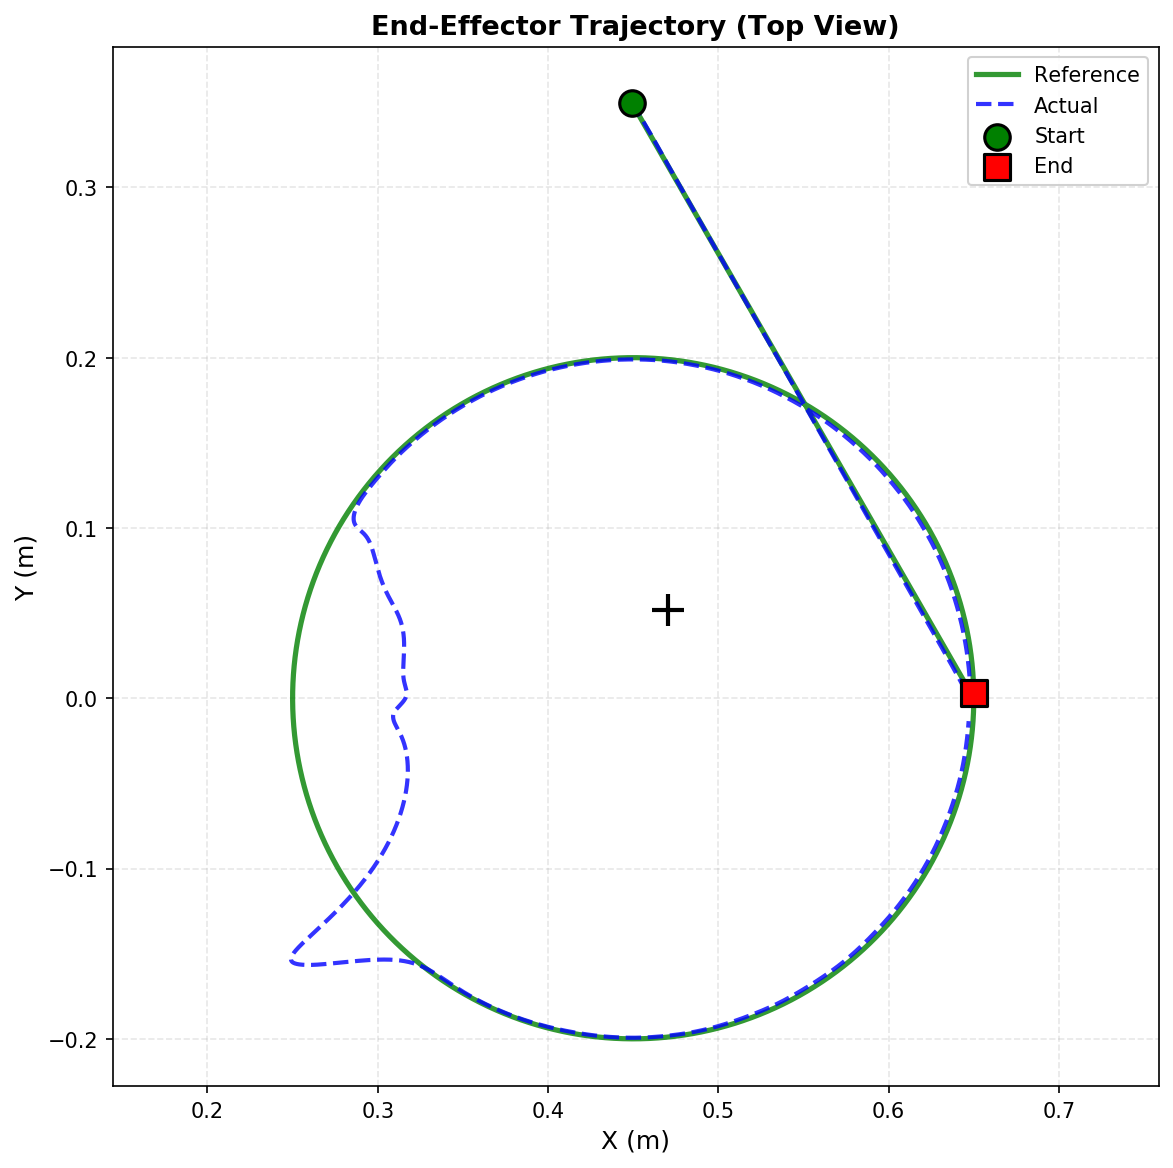
\includegraphics[width=0.7\columnwidth]{images/trajectory_xy.png}
	\caption{Top view of circular cleaning trajectory in XY plane}
	\label{fig:trajectory_xy}
\end{figure}

\begin{figure}[h]
	\centering
	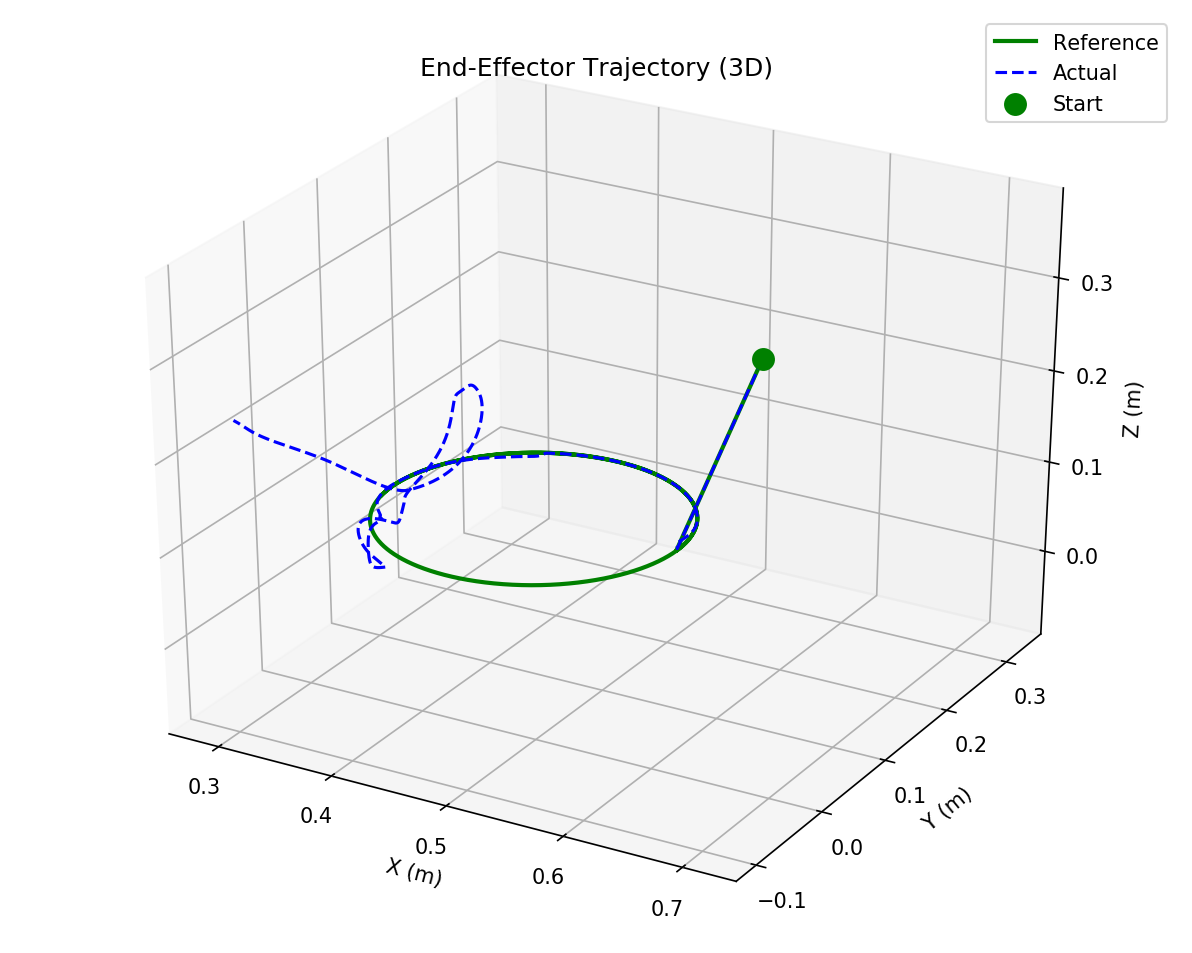
\includegraphics[width=\columnwidth]{images/trajectory_no_opt_3d.png}
	\caption{Top view of circular cleaning trajectory in 3D without manipulability optimization}
	\label{fig:trajectory_no_opt_3d}
\end{figure}

\subsubsection{Tracking Error Analysis}
Fig.~\ref{fig:tracking_errors} presents the time evolution of position and orientation tracking errors. The position error remains consistently below 2 mm (with some spikes close to singularity zones), while orientation error stays under 0.22 degrees.
\begin{figure}[h]
	\centering
	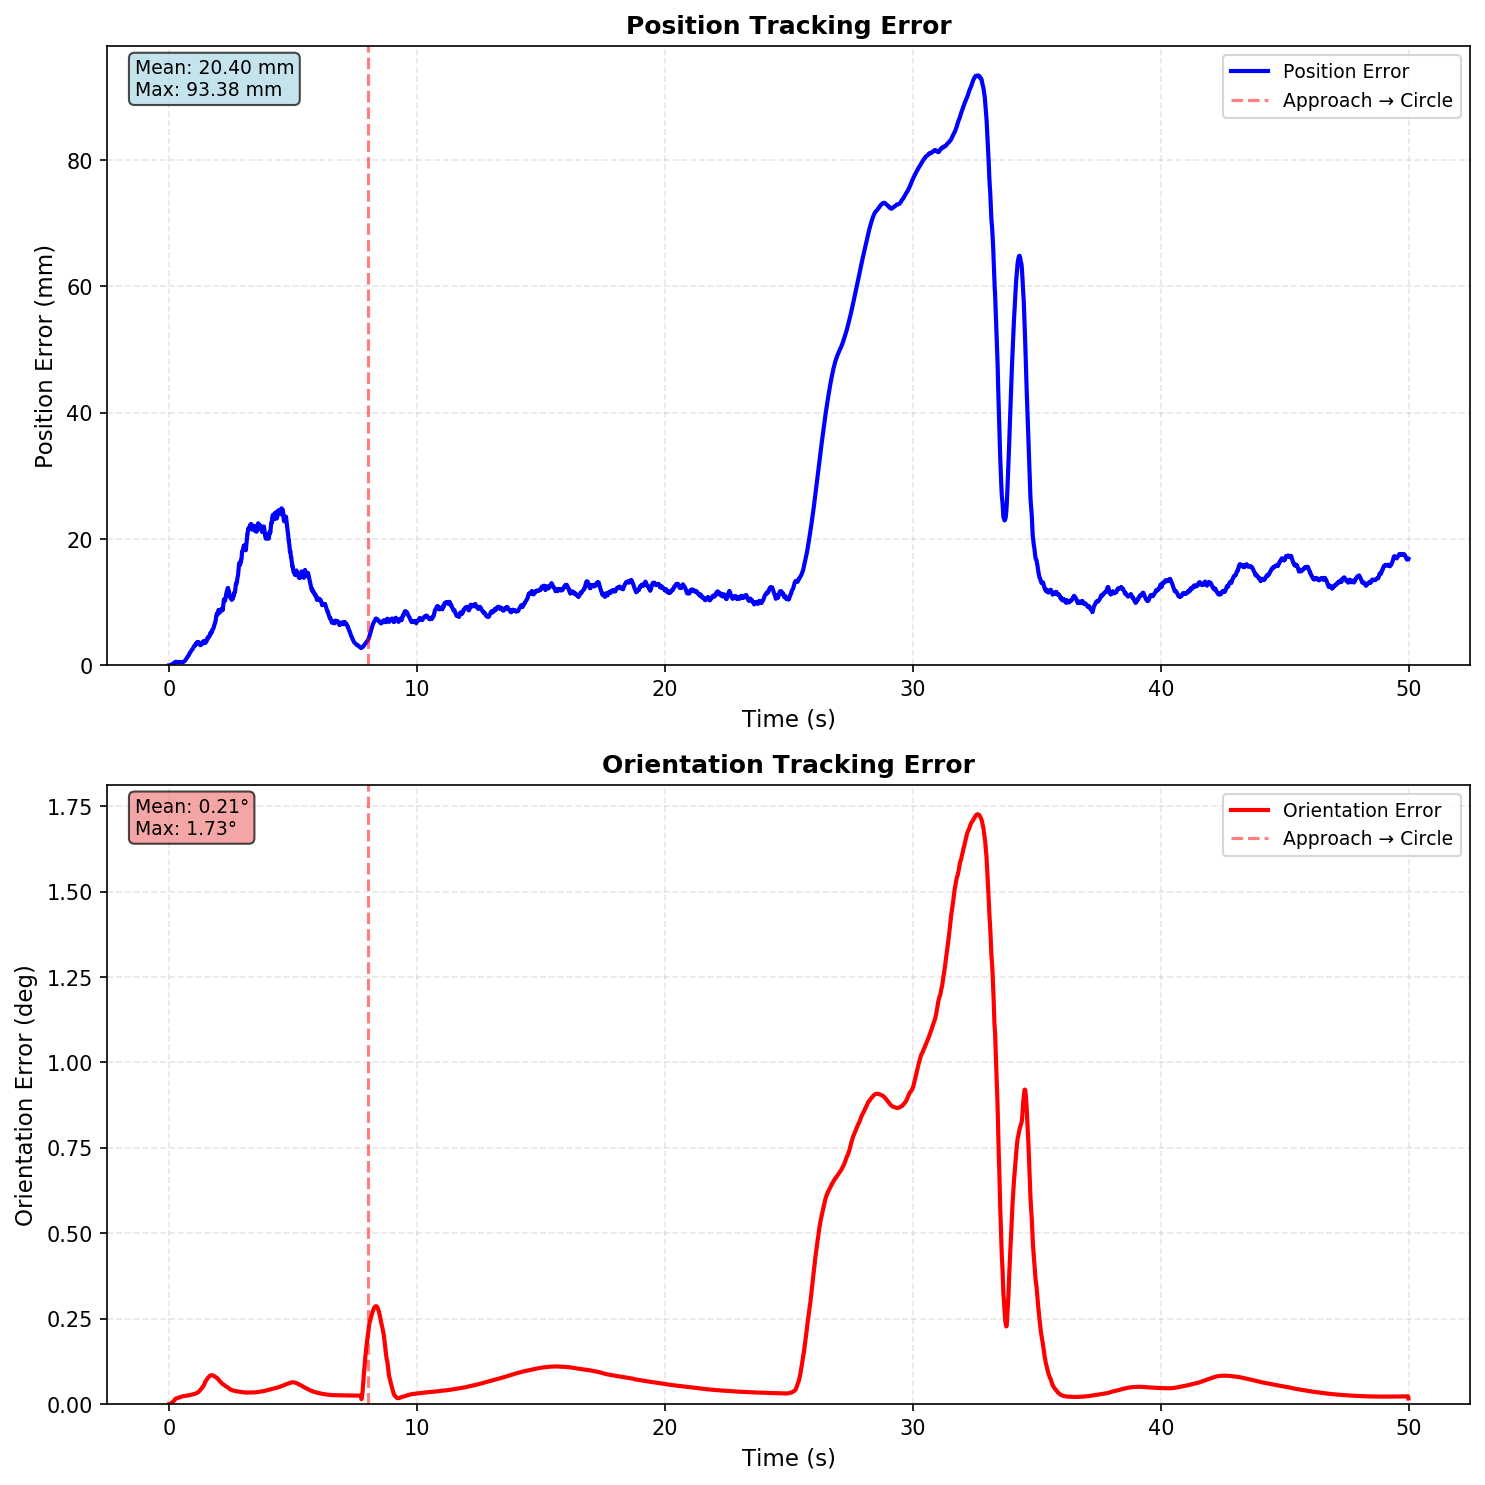
\includegraphics[width=0.9\columnwidth]{images/tracking_errors.png}
	\caption{Position and orientation tracking errors over time}
	\label{fig:tracking_errors}
\end{figure}

\subsubsection{Manipulability Optimization}
The effectiveness of null-space optimization is clearly demonstrated in Fig.~\ref{fig:joint_torques}. With manipulability optimization, the robot maintains healthy manipulability values (0.06-0.07) throughout the trajectory, while the baseline system experiences dramatic drops to near-singular configurations (0.02-0.03).

\subsubsection{Joint Torque Analysis}
Fig.~\ref{fig:joint_torques} shows the joint torque requirements for all 8 DOFs during the cleaning motion. The torques remain within safe limits, with the platform joints (0-1) and shoulder/elbow joints (3-4) carrying the primary load due to their significant contribution to end-effector positioning.

\begin{figure}[h]
	\centering
	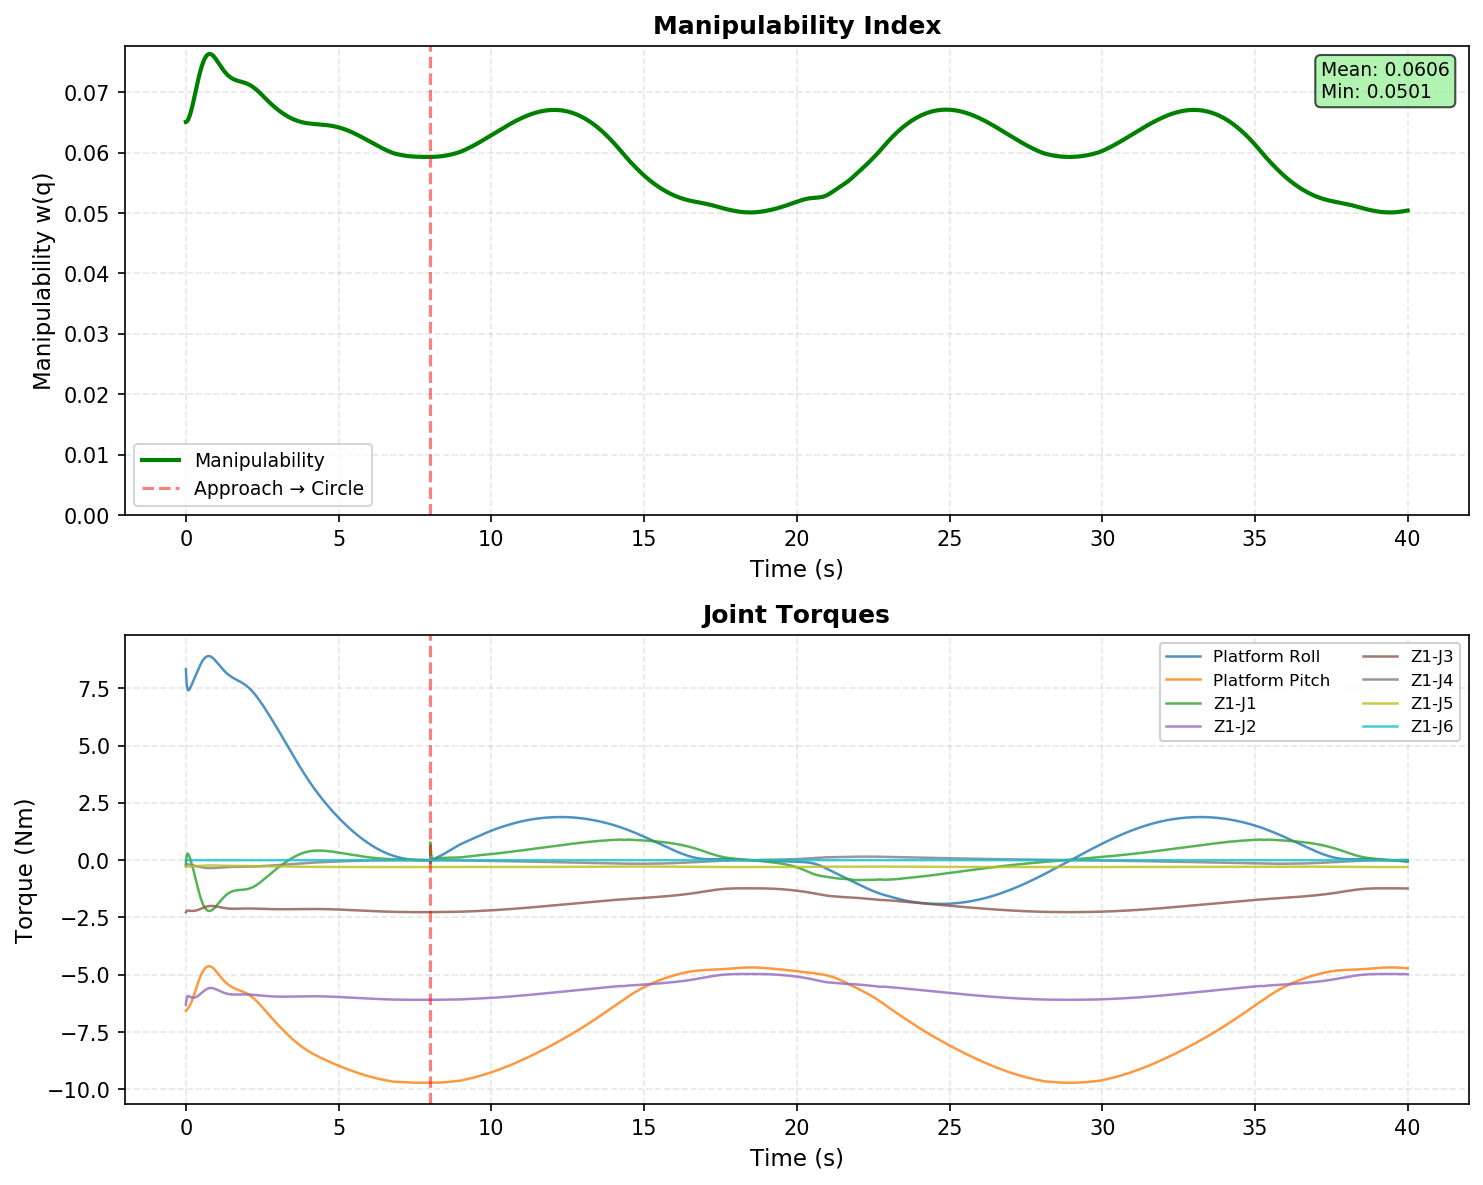
\includegraphics[width=\columnwidth]{images/performance.png}
	\caption{Robot manipulability and joint torques for all 8 DOFs}
	\label{fig:joint_torques}
\end{figure}

\subsubsection{The role of manipulability}
Fig.~\ref{fig:screenshot_without_manip} reveals the catastrophic tracking failure without manipulability optimization. The robot configuration drifts toward kinematic singularities, leading to complete loss of tracking capability and tool orientation control.

\begin{figure}[h]
	\centering
	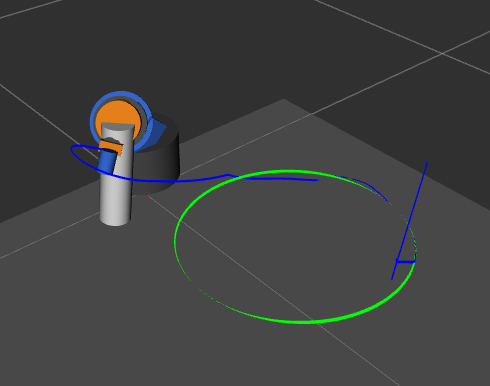
\includegraphics[width=0.7\columnwidth]{images/no_manipulability.png}
	\caption{Robot motion without manipulability optimization - tracking failure due to singularities}
	\label{fig:screenshot_without_manip}
\end{figure}

\subsubsection{Performance Impact Analysis}
The performance degradation without null-space optimization manifests through several critical failure modes:

\begin{itemize}
    \item \textbf{Manipulability Collapse}: Drop from 0.06-0.07 (healthy) to 0.02-0.03 (near-singular)
    \item \textbf{Tracking Degradation}: Position errors explode from mm to cm scale
    \item \textbf{Orientation Loss}: Complete failure to maintain tool perpendicularity
    \item \textbf{Control Instability}: Pseudoinverse singularity prevents valid joint commands
\end{itemize}

Comparing Fig.~\ref{fig:robot_main} and Fig.~\ref{fig:screenshot_without_manip} clearly demonstrates this phenomenon: the optimized system maintains stable circular tracking throughout the entire cleaning cycle, while the non-optimized system suffers catastrophic failure near singular configurations, making it unsuitable for practical cleaning applications.

\section{AI Usage}
Throughout my project, artificial intelligence tools were utilized to enhance both my theoretical understanding of class lectures and practical implementation. AI assistance was instrumental in my study of robotics concepts from lectures including redundant manipulator theory, task-space control principles, and singularity analysis. The AI guidance helped me identify optimal implementation approaches, particularly the application of Yoshikawa's manipulability measures for redundancy resolution and the selection of quintic polynomial trajectories for smooth approach phase. This AI-enhanced learning process enabled my deeper comprehension of complex mathematical foundations and their practical applications in robotic control systems, ultimately leading to my more informed design decisions and effective implementation strategies.

\section{Conclusion}

This project demonstrates the design and implementation of a redundant 8-DoF cleaning robot with advanced task-space control capabilities. 
The integration of a pan-tilt platform with a robotic arm showcases the benefits of kinematic redundancy in service robotics applications while null-space optimization strategy effectively exploits the additional degrees of freedom to enhance robot conditioning while maintaining primary task performance.

\begin{thebibliography}{99}
\bibitem{yoshikawa1985}
T. Yoshikawa, ``Manipulability of robotic mechanisms,'' \emph{The International Journal of Robotics Research}, vol. 4, no. 2, pp. 3--9, 1985. [Online]. Available: https://tsuneo-yoshikawa.my.coocan.jp/PDF-of-Papers/1985-EP2.pdf

\bibitem{unitree}
Unitree Robotics, ``Z1 Technical Specifications,'' 2023. [Online]. Available: https://www.unitree.com/z1
\end{thebibliography}

\end{document}
